\documentclass[tikz,border=2pt]{standalone}
\usepackage{amsmath}
\usetikzlibrary{arrows.meta}
\definecolor{bg}{HTML}{171D2B}
\definecolor{acc}{HTML}{F7B538}
\begin{document}
\pagecolor{bg}
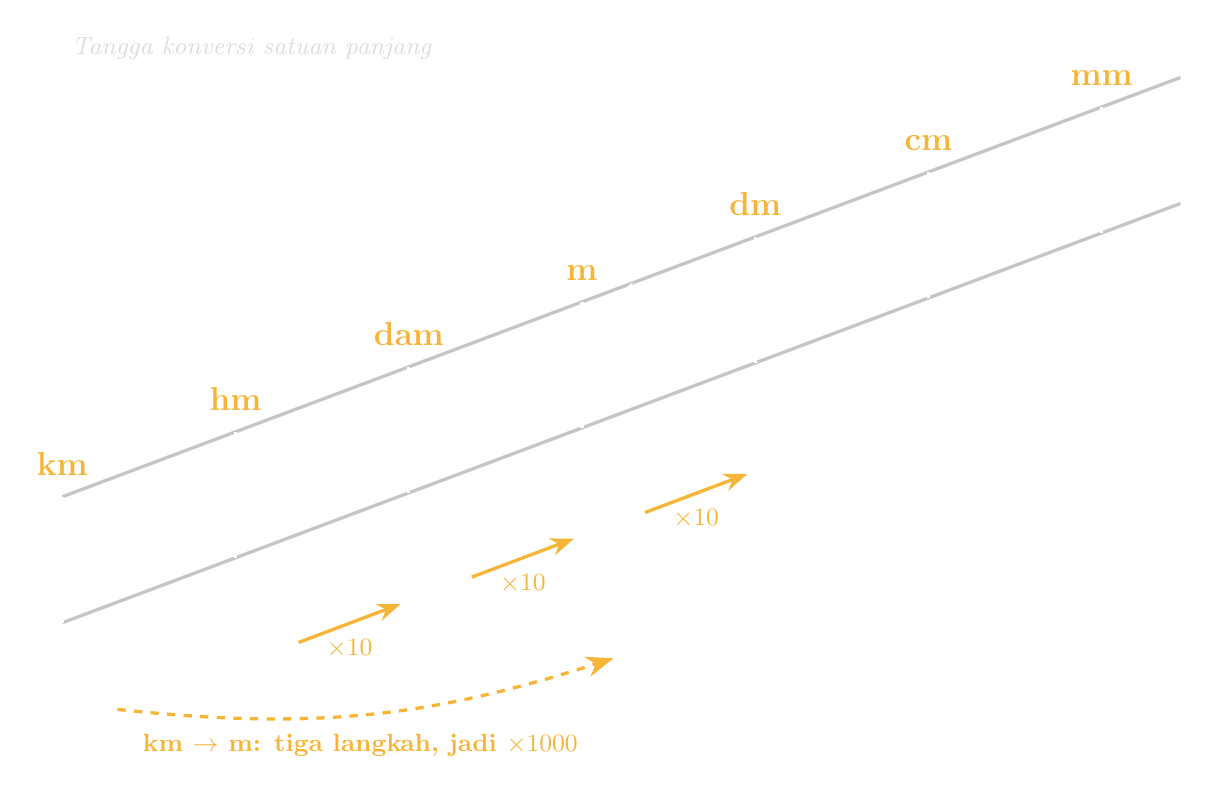
\begin{tikzpicture}[
  scale=1.0,
  text=white,
  unit/.style={font=\bfseries\large, text=acc},
  down/.style={-{Stealth[length=3mm]}, draw=acc, very thick},
  up/.style={-{Stealth[length=3mm]}, draw=white, very thick},
  jump/.style={-{Stealth[length=3.5mm]}, draw=acc, very thick, dashed},
]

% dua garis miring tangga (kemiringan 0.375), sedikit melebihi anak tangga terakhir
\draw[draw=white!75!bg, very thick] (0,0) -- (14.2,5.325);
\draw[draw=white!75!bg, very thick] (0,1.6) -- (14.2,6.925);

% anak tangga: garis vertikal penuh menghubungkan dua rel
% pada x = i*2.2: rel bawah y = 0.825*i, rel atas y = rel bawah + 1.6
\foreach \i/\sat in {0/km,1/hm,2/dam,3/m,4/dm,5/cm,6/mm} {
  \draw[draw=white, very thick] ({\i*2.2},{0.825*\i}) -- ({\i*2.2},{0.825*\i+1.6});
  \node[unit, anchor=south] at ({\i*2.2},{0.825*\i+1.75}) {\sat};
}

% panah turun (kali 10) di celah antar anak tangga, di bawah rel bawah
\draw[down] (3.0,-0.25) -- (4.3,0.24) node[midway, below=2pt, text=acc, font=\small] {$\times 10$};
\draw[down] (5.2,0.58) -- (6.5,1.07) node[midway, below=2pt, text=acc, font=\small] {$\times 10$};
\draw[down] (7.4,1.40) -- (8.7,1.89) node[midway, below=2pt, text=acc, font=\small] {$\times 10$};

% panah naik (bagi 10) di celah antar anak tangga, di atas rel atas
\draw[up] (8.3,4.6) -- (7.0,4.11) node[midway, above=2pt, text=white, font=\small] {$:\!10$};

% panah lompat km -> m dengan anotasi
\draw[jump] (0.7,-1.1) to[bend right=12] (7.0,-0.45);
\node[text=acc, font=\small\bfseries, anchor=west] at (0.9,-1.55) {km $\rightarrow$ m: tiga langkah, jadi $\times 1000$};

% judul kecil
\node[anchor=west, text=white!85!bg, font=\small\itshape] at (0,7.3) {Tangga konversi satuan panjang};

\end{tikzpicture}
\end{document}
